
\documentclass[a4paper,10pt]{article}
\usepackage{tikz}
\usetikzlibrary{arrows.meta,positioning}


% passe en mode large sur la page A4
\usepackage{a4wide} 

% document francisé
\usepackage[polutonikogreek,english,francais]{babel} 

% permet la frappe de caracteres accentues (sur macOS)
%\usepackage[utf8x]{inputenc} 

\usepackage{graphicx,float,subcaption} % figure et placement de figure
\usepackage[top=10mm, bottom=10mm, left=20mm, right=20mm]{geometry}

\usepackage[linesnumbered,frenchkw,ruled,french]{algorithm2e}

\usepackage{verbatim}
\usepackage{fancyvrb}
\usepackage[T1]{fontenc}
%\usepackage{graphicx}
%\usepackage{grffile}
%\usepackage{longtable}
%\usepackage{wrapfig}
%\usepackage{rotating}
%\usepackage[normalem]{ulem}
%\usepackage{amsmath}
%\usepackage{textcomp}
%\usepackage{amssymb}
%\usepackage{capt-of}
\usepackage{hyperref}% \documentclass[a4paper,11pt]{article}
%\usepackage[margin=2cm]{geometry}
\usepackage[utf8]{inputenc}

\usepackage{color}
\usepackage{xcolor}

\usepackage[]{amsmath,amsfonts,amssymb,stmaryrd,amsthm}
\let\oldemptyset\emptyset
\let\emptyset\varnothing
%\usepackage{fullpage}
%\usepackage{multirow}
%\usepackage[rounded]{syntax}
%\usepackage[section]{placeins}
\newtheorem{example}{Exemple} %%% modifier ici si on veut en fr/en

\usepackage{musixtex}

\usepackage{todonotes}
\usepackage{listings} 


\usepackage{listings}
\usepackage{inconsolata} % very nice fixed-width font included with texlive-full
%\usepackage[usenames,dvipsnames]{color} % more flexible names for syntax highlighting colors

\definecolor{chameleond}{HTML}{4E9A06}
\definecolor{skyblued}{HTML}{204A87}
\definecolor{darkgreen}{HTML}{006400}

%\usepackage[usenames,dvipsnames]{color} % more flexible names for syntax highlighting colors


\lstset{
basicstyle=\ttfamily, 
columns=fullflexible, % make sure to use fixed-width font, CM typewriter is NOT fixed width
numbers=left, 
numberstyle=\small\ttfamily\color{gray},
stepnumber=1,              
numbersep=10pt, 
numberfirstline=true, 
numberblanklines=true, 
tabsize=4,
lineskip=-1.5pt,
extendedchars=true,
breaklines=true,        
keywordstyle=\color{skyblued}\bfseries,
identifierstyle=, % using emph or index keywords
commentstyle=\sffamily\color{darkgreen},
stringstyle=\color{chameleond},
showstringspaces=false,
showtabs=false,
upquote=false,
texcl=true % interpet comments as LaTeX
}


\lstset{literate=
  {α}{{$\alpha$}}1 {Δ}{{$\Delta$}}1
  {á}{{\'a}}1 {é}{{\'e}}1 {í}{{\'i}}1 {ó}{{\'o}}1 {ú}{{\'u}}1
  {Á}{{\'A}}1 {É}{{\'E}}1 {Í}{{\'I}}1 {Ó}{{\'O}}1 {Ú}{{\'U}}1
  {à}{{\`a}}1 {è}{{\`e}}1 {ì}{{\`i}}1 {ò}{{\`o}}1 {ù}{{\`u}}1
  {À}{{\`A}}1 {È}{{\'E}}1 {Ì}{{\`I}}1 {Ò}{{\`O}}1 {Ù}{{\`U}}1
  {ä}{{\"a}}1 {ë}{{\"e}}1 {ï}{{\"i}}1 {ö}{{\"o}}1 {ü}{{\"u}}1
  {Ä}{{\"A}}1 {Ë}{{\"E}}1 {Ï}{{\"I}}1 {Ö}{{\"O}}1 {Ü}{{\"U}}1
  {â}{{\^a}}1 {ê}{{\^e}}1 {î}{{\^i}}1 {ô}{{\^o}}1 {û}{{\^u}}1
  {Â}{{\^A}}1 {Ê}{{\^E}}1 {Î}{{\^I}}1 {Ô}{{\^O}}1 {Û}{{\^U}}1
  {œ}{{\oe}}1 {Œ}{{\OE}}1 {æ}{{\ae}}1 {Æ}{{\AE}}1 {ß}{{\ss}}1
  {ű}{{\H{u}}}1 {Ű}{{\H{U}}}1 {ő}{{\H{o}}}1 {Ő}{{\H{O}}}1
  {ç}{{\c c}}1 {Ç}{{\c C}}1 {ø}{{\o}}1 {å}{{\r a}}1 {Å}{{\r A}}1
  {€}{{\EUR}}1 {£}{{\pounds}}1
}

% \lstset{language=bash,
% stringstyle=\ttfamily,
% basicstyle=\footnotesize, 
% showstringspaces=false,
% breaklines=true,
% }

\lstdefinestyle{numbers} {numbers=left, stepnumber=5, numberstyle=\tiny, numbersep=10pt}
% \lstdefinestyle{lc3} {language=[x86masm]Assembler,style=numbers,frame=lines,showstringspaces=false,keywords={BR,LD,BRz,BRn,BRzp,BRnz,BRnzp,LEA,HALT,RET,.END,.ORIG,.FILL,.STRINGZ,PUTS,ADD,AND,OR,OUT,NOT,LDR,STR,JSR,NOP,GETC},showstringspaces=false,keepspaces=true,flexiblecolumns=true,deletekeywords={end}}

\lstdefinestyle{target}
{language=[x86masm]Assembler,style=numbers,frame=lines,showstringspaces=false,keywords={add,
  jump, snif,call,return,.string,.reserve,.word,.set,.align16,letl,leth,.let,and,or,wmem,rmem,asr,xor,sub,sgt,sle,slt,slt},showstringspaces=false,keepspaces=true,flexiblecolumns=true,deletekeywords={end},breaklines=true}



%\definecolor{chameleond}{HTML}{4E9A06}
%\definecolor{skyblued}{HTML}{204A87}


\lstdefinestyle{digmips} {language=[x86masm]Assembler,style=numbers,frame=lines,showstringspaces=false,keywords={add,sub,ld,ldi,ble,j,jmp,st},showstringspaces=false,keepspaces=true,flexiblecolumns=true,deletekeywords={end},keywordstyle=\color{skyblued},commentstyle=\color{red}\bf,morecomment=[l][\color{red}]{//}}


\lstdefinestyle{lc3} {language=[x86masm]Assembler,style=numbers,frame=lines,showstringspaces=false,keywords={BR,LD,BRz,BRn,BRzp,BRnz,BRnzp,LEA,HALT,RET,.END,.ORIG,.FILL,.STRINGZ,PUTS,ADD,AND,OR,OUT,NOT,LDR,STR,JSR,NOP,GETC},showstringspaces=false,keepspaces=true,flexiblecolumns=true,deletekeywords={end}}


\lstdefinelanguage{[Objective]Caml}
{basicstyle=\ttfamily,
keywordstyle=\itshape\bfseries,
identifierstyle=,
stringstyle=\itshape,
commentstyle=\itshape,
flexiblecolumns=true,
escapechar=\%}

\lstdefinelanguage{julia}
{
  keywordsprefix=\@,
  morekeywords={
    exit,whos,edit,load,is,isa,isequal,typeof,tuple,ntuple,uid,hash,finalizer,convert,promote,
    subtype,typemin,typemax,realmin,realmax,sizeof,eps,promote_type,method_exists,applicable,
    invoke,dlopen,dlsym,system,error,throw,assert,new,Inf,Nan,pi,im,begin,while,for,in,return,
    break,continue,macro,quote,let,if,elseif,else,try,catch,end,bitstype,ccall,do,using,module,
    import,export,importall,baremodule,immutable,local,global,const,Bool,Int,Int8,Int16,Int32,
    Int64,Uint,Uint8,Uint16,Uint32,Uint64,Float32,Float64,Complex64,Complex128,Any,Nothing,None,
    function,type,typealias,abstract
  },
  sensitive=true,
  morecomment=[l]{\#},
%  morecomment=[s]{# =}{=#},
  morestring=[b]',
  morestring=[b]" 
}

\lstdefinelanguage{cplus}
{
        frame=lines,
	language=C++,
	basicstyle=\tt,
        morecomment=[l][\color{magenta}]{\#},
	keywordstyle=\color{chameleond},
	identifierstyle=\color{black},
        stringstyle=\color{skyblued},
        commentstyle=\color{red},
	tabsize=4,
}


\lstdefinelanguage{mypython}
{
%        frame=lines,
	language=Python,
	basicstyle=\tt,
        morecomment=[l][\color{magenta}]{\#},
	keywordstyle=\color{chameleond},
	identifierstyle=\color{black},
        stringstyle=\color{skyblued},
        commentstyle=\color{red},
	tabsize=4,
        breaklines=true,
}


\lstdefinelanguage{flexbison}
{
        frame=lines,
	language=C,
	basicstyle=\tt,
        keywords={yylex,yyparse,yyline,yytext,yyin},
        morecomment=[l][\color{magenta}]{\#,},
	keywordstyle=\color{chameleond},
	identifierstyle=\color{black},
        stringstyle=\color{skyblued},
        commentstyle=\color{red},
	tabsize=4,
}


\lstdefinelanguage{antlr}
{
%  frame=lines,
  language=Java,
  basicstyle=\tt\scriptsize,
  breaklines=true,%                                      allow line breaks
  moredelim=[s][\color{blue!50!black}\ttfamily]{'}{'},% single quotes in green
  moredelim=*[s][\color{black}\ttfamily]{options}{\}},%  options in black (until trailing })
  commentstyle={\color{gray}\itshape},%                  gray italics for comments
  morecomment=[l]{//},%                                  define // comment
  emph={%
    STRING%                                            literal strings listed here
  },emphstyle={\color{blue}\ttfamily},%              and formatted in
                                %              blue
  keywords={grammar,header,members,skip},
  alsoletter={:,|,;},%
  morekeywords={:,|,;},%                                 define the special characters
  keywordstyle={\color{chameleond}},%                         and format them in black
}


\lstdefinelanguage{mycaml}
{       language=Caml,
        upquote=true,
        columns=flexible,
        keepspaces=true,
        breakindent=0pt,
        basicstyle=\ttfamily,
        breaklines=true,
        keywordstyle=\color{red},
        commentstyle=\color{darkgreen},
        tabsize=2,
        escapechar=\%,
        escapebegin=\color{blue}
        }

\lstdefinelanguage{myhaskell}
{       language=Haskell,
        upquote=true,
        columns=flexible,
        keepspaces=true,
        breakindent=0pt,
        basicstyle=\ttfamily\scriptsize,
        breaklines=true,
        keywordstyle=\color{red},
        commentstyle=\color{darkgreen},
        tabsize=2,
        escapeinside={!}{!},
        escapebegin=!\endgraf\color{gray},
        }



\newcommand\ocamli[1]{\lstinline[language=mycaml,basicstyle=\ttfamily\normalsize]{#1}}
\newcommand\llvminline[1]{\lstinline[language=LLVM,basicstyle=\ttfamily\normalsize]{#1}}
\newcommand\llvmfile[1]{\lstinputlisting[language=LLVM]{#1}}

\lstnewenvironment{llvmc}{
  \lstset{language=llvm,mathescape,
    basicstyle=\ttfamily\small,
    aboveskip={0\baselineskip},
    belowskip=0\baselineskip
  }}{}


\lstdefinelanguage{lustre}
{
  basewidth={0.5em,0.5em},
  % list of keywords
  morekeywords={
    pre,
    fby,
    ->,
    current,
    when,
    node, 
    returns,
    let,
    tel,
    var,
    if,
    then,
    int,
    bool,
  },
  sensitive=false, % keywords are not case-sensitive
  escapeinside={!}{!},          % if you want to add LaTeX within your code
  morecomment=[l]{//}, % l is for line comment
  morecomment=[s]{/*}{*/}, % s is for start and end delimiter
  morestring=[b]", % defines that strings are enclosed in double quotes
  basicstyle=\ttfamily,
  keywordstyle=\bfseries\color{blue!80!black},
  keywordstyle=[2]\bfseries\color{red!50!white},
  commentstyle=\itshape\color{purple!40!black},
  %identifierstyle=\color{blue!80!black},
  stringstyle=\color{orange}
}


\newcommand{\arthur}[1]{\textcolor{violet}{\textsc{#1}}}
\newcommand{\prof}[1]{\textcolor{red}{\textsc{#1}}}
\newcommand{\mehdi}[1]{\textcolor{white}{#1}}


% individualisation des parametres de la page
\parskip8pt
\setlength{\topmargin}{-25mm}
\setlength{\textheight}{250mm}

%
% -----------------------------------------------------------------------------------------------------------------------------------------------------
%
%% Packages pour la preuve 
\theoremstyle{plain}
\newtheorem*{thm}{Théorème}
\usepackage{stmaryrd}
\newenvironment{definition}[1][Définition]{\begin{trivlist}
  \item[\hskip \labelsep {\bfseries #1}]}{\end{trivlist}}
%\usepackage{biblatex}
%\addbibresource{combi.bib}


\begin{document}

\lstset{language=julia}

% paramètres des graphs
\tikzstyle{fleche}=[->,thick,>=latex]
\tikzstyle{noeud}=[circle,fill=violet!20]
\tikzstyle{legende}=[scale = 0.7,pos=0.59]


~
\vspace{50mm}
       {\large
         \begin{center}
           Université de Nantes --- UFR Sciences et Techniques\\
           Master informatique parcours ``optimisation en recherche opérationnelle (ORO)''\\
           Année académique 2018-2019
           \vspace{30mm}
           
           { \LARGE
             
             Rapport de TER\\
             \vspace{5mm}
             
             {\huge \textbf{Implémentation Julia de l'algorithme simplexe multi-objectif avec la forme révisé du simplexe et la décomposition LU}}
             \vspace{5mm}
             
             Stagiaire : Arthur \textsc{Gontier} \\
             Encadrants : Anthony \textsc{Przybylski}$^1$, Xavier \textsc{Gandibleux}$^2$
             \vspace{50mm}
             
             \today
           }  
         \end{center}
       }

\begin{abstract}
  \arthur{On fais une abstract ?}
\end{abstract}

\vfill
\break

\tableofcontents

\vfill
\break

\section{Introduction}\arthur{a refaire\\}
Nous savons aujourd'hui résoudre beaucoup de problèmes mono-objectifs et il existe de plus en plus d'algorithmes pour les problèmes bi-objectifs. Mais les solutions apportées aux problèmes à plus de trois objectifs sont rares du fait non pas de leur complexité mais par un manque de propriétés à exploiter. Si les algorithmes bi-objectifs peuvent parcourir les solutions paréto-optimales de manière linéaire, cela devient plus difficile pour plus de trois objectifs même si la résolution du problème reste une somme pondérée. On se retrouve alors obligé d'énumérer en évitant les cyclages toutes les bases qui donnent une solution non-dominée de manière un peut brut.\\
L'objet de ce travail encadré de recherche est donc d'abord la compréhension de l'algorithme du simplexe multicritère puis son implémentations avec la forme révisé du simplexe et la décomposition LU.\\
Ce projet est donc parti du Chapitre 7 : ``multicriteria simplexe'' du livre de Matthias Ehrgott ``Multicriteria optimization'' \cite{ehrgott2005multicriteria} 

\section{Définitions et notations}
\subsection{Programme linéaire}
Un programme linéaire est la formulation d'un problème avec une fonction objectif $x^Tc$ et des contraintes $Ax\leq b$ sous forme de fonctions linéaires. La solution optimale $x$ doit maximiser ou minimiser la valeur de la fonction objectif $x^Tc$ tout en respectant les contraintes $Ax\leq b$. On remarque que les contraintes sont des demi-espaces. Ensemble, elles délimitent une enveloppe convexe, un polytope dans lequel les solution sont acceptés. Il se peut que l'intersection des demi-espaces donne un polytope vide. On dit alors que le problème n'a pas de solution. s'il n'est pas vide, les solutions qui sont dans le polytope sont appelés solutions réalisables. Comme la fonction objectif est une fonction linéaire, elle traverse le polytope et donc la meilleure solution du problème est sur le bord du polytope dans la direction de la fonction objectif. Elle est appelée solution optimale.

\begin{figure}[htb!]
  \centering
  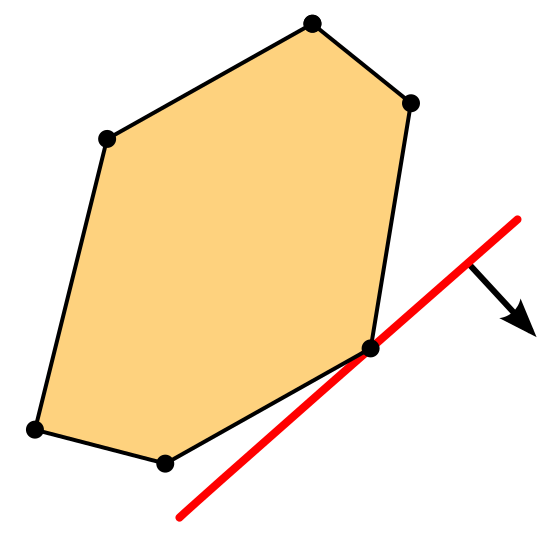
\includegraphics[scale=0.3]{doc/polytope.png}
  \caption{Exemple de polytope, de fonction objectif et de solution optimale}
  \label{fig:polytope}
\end{figure}

Pour les notation, $^T$ est la transposé d'un vecteur, $x$ est une solution, $c$ le vecteur des coûts de la fonction objectif, $A$ est la matrice des coûts des contraintes et $b$ le vecteur des valeurs que ces contraintes ne doivent pas dépasser. On peut alors écrire le programme linéaire comme suit : $$ min \{ c^Tx : Ax \geq b,x \geq 0 \} $$
Si on a $n$ le nombre de variables et $m$ le nombre de contraintes, on a : $$x\in \mathbb{R}^n ; c\in \mathbb{R}^n ; A\in \mathbb{R}^{n \times m} ; b\in \mathbb{R}^m$$

\subsection{Algorithme du simplexe}
L'algorithme du simplexe permet de résoudre des programmes linéaires de manière très efficace en pratique malgré sa complexité exponentielle. Il se déroule en deux phases distinctes :
\begin{itemize}
\item La \textbf{phase une} consiste à vérifier que les contraintes ne sont pas impossibles à satisfaire et à trouver un point dans la région admissibles du problème. Elle est identique pour le simplexe multi-objectif.
\item Si le problème n'est pas impossible, on entame la \textbf{phase deux}. L'idée est de se déplacer sur les arrêtes du polytope jusqu'à trouver la solution optimale. Pour cela, on ajoute au problème une variable d'écart pour chaque contrainte. Cette variable modélise l'écart entre la solution courante x et la contrainte. Quand cette variable est égale à zéro, cela signifie que la solution est au bord de la contrainte. On dit que la contrainte est saturée et que les variables d'écart sont en base. L'algorithme consiste donc à chercher la combinaison de variables en bases qui donnent la meilleure solution. Pour ceci, il fait des pivot de gauss pour se déplacer de base en base.
\end{itemize}

\subsubsection{pivot de gauss}
Un pivot de gauss, dans le cas du simplexe consiste à faire entrer une variables $X_j$ en base et à choisir une variable sortante $X_s$. ces choix se font toujours en fonction le l'objectif du problème. On ajoute la variable qui augmentera le plus notre solution et on retire la variable d'écart qui saturera le plus tard possible pour faire le plus grand déplacement possible vers la solution optimale.
Par exemple si on prend le tableau simplexe suivant :

\begin{equation}
  \begin{bmatrix}
    \begin{array}{c|ccccc|c}
      \mehdi{.} & x_1 & x_2 & x_3 & x_4 & x_5 & b \\ \hline
      z  & 3 & 2 & 0 & 0 & 0 & 0 \\ \hline
      x_3 & 2 & 1 & 1 & 0 & 0 & 6 \\
      x_4 & 1 & 1 & 0 & 1 & 0 & 4 \\
      x_5 & 0 & 1 & 0 & 0 & 1 & 3 \\
    \end{array}
  \end{bmatrix}
\end{equation}

On souhaite faire entrer La variable $X_1$ dans la base car elle a la plus grande valeur dans la foncions objectif ($z$). 

On cherche donc la variable en base qui permettra d'augmenter le plus possible la valeur de la fonction objectif avant de saturer. On calcul la division du vecteur $b$ par la colonne de $X_1$ pour trouver le meilleur ratio. Dans ce cas on a $6/2$ et $4/1$ donc la variable sortante est $X_3$

On effectue le pivot de gauss et on obtient le tableau suivant : 
\begin{equation}
  \begin{bmatrix}
    \begin{array}{c|ccccc|c}
      \mehdi{.} & x_1 & x_2 & x_3 & x_4 & x_5 & b \\ \hline
      z  & 0 & 1/2 & -3/2 & 0 & 0 & -9 \\ \hline
      x_1 & 1 & 1/2 & 1/2 & 0 & 0 & 3 \\
      x_4 & 0 & 1/2 & -1/2 & 1 & 0 & 1 \\
      x_5 & 0 & 1 & 0 & 0 & 1 & 3 \\
    \end{array}
  \end{bmatrix}
\end{equation}

On répète l'algorithme jusqu'à ce qu'il n'y ai plus de valeurs positives dans la fonction objectif $z$.

\subsection{Forme révisée du simplexe}
L'algorithme du simplexe sous sa forme classique demande de calculer une suite de tableaux simplexe. En théorie cela ne pose aucun problèmes mais dans la pratique ces calculs en génèrent des imprécisions numériques qui se propagent de tableau en tableau. Et si le problème est trop long à résoudre, on peut finir avec des tableaux complètement erronés.

C'est pourquoi nous nous intéresseront à la forme révisée du simplexe pour calculer ces tableaux

La forme révisée du simplexe permet de calculer un tableau simplexe dans n'importe quelle base à partir des données d'origine du problème.
Par exemple si on reprend la formulation du problème : $$ min \{ c^Tx : Ax \geq b,x \geq 0 \} $$
Et qu'on note $B$ la base dans laquelle on veut trouver le prochain pivot.

On recalcule les coûts réduits, cet à dire les valeurs de la fonction objectif avec la formule : $$c^T-c_B^TA_B^{-1}A$$

La colonne de la variable $X_j$ est donnée par la formule : $$A_B^{-1}A$$

Et le vecteur $b$ par la formule $$A_B^{-1}b$$

Ces informations suffisent pour détecter la variable entrante et trouver la variable sortante du prochain pivot de gauss.

On remplace donc une suite de tableaux simplexe par un calcul de la matrice inverse $A_B^{-1}$ pour avoir directement les valeurs qui nous intéressent.\\
%cf diapo distantiel opti combi et discrète

\subsection{Décomposition LU}
La forme révisé remplace la suite de tableau par le calcul d'une matrice inverse $A_B^{-1}$ mais si nos problèmes se modélisent souvent par des matrice creuses les matrices inverses de ces dernières ne le sont généralement pas.

La décomposition LU permet de simplifier grandement les calculs matriciels de la forme révisé du simplexe. En effet plutôt que de calculer une matrice inverse, on calcule la décomposition LU de la matrice $A_B$. Cette méthode décompose la matrice $A_B$ en deux matrices $L$ et $U$ qui sont respectivement des matrices triangulaires infèrieure et triangulaires supèrieure.

Une fois la décomposition LU calculée, on en déduit les coûts réduits, la colonne de la variable $X_j$, et le vecteur $b$ avec des systèmes d'équation. Ces systèmes d'équations sont très simples grâce à la nature triangulaire des matrices $L$ et $U$.

Ces deux méthodes permettent d'avoir une implémentation d'algorithme moins encline à générer des imprécisions numériques. Elles sont très utilisées dans les simplexe des solveurs.\\

\subsection{Optimisation multi-objectif}
Il arrive bien souvent que l'on souhaite optimiser un problème en prenant en compte un ou plusieurs autres objectifs. Par exemple on pourrais vouloir acheter un bonbon par rapport à sa taille et son prix. On voudrais prendre en compte les deux en même temps et cela malgré le fait que ces objectifs sont contradictoires. Pour résoudre ce problème, on maximiserai la taille du bonbon tout en minimisant son prix.

On indice des vecteurs de ces objectifs $c_1...c_n$ et on les met tous dans une matrice $C$. On peut alors noter le MOLP comme suit : $$ min \{ Cx : Ax \geq b,x \geq 0 \} $$

\subsubsection{Optimalité et Dominance}\arthur{à refaire}
On se retrouve avec des solution que l'on ne peut pas comparer\footnote{Un peu comme dans un treillis}. Comment décider entre un petit bonbon pas cher et un gros bonbon très cher. Il existe plusieurs définition de dominances mais ici on ne s'intéressera qu'aux solution dont il n'existe pas d'autre solution admissibles qui leur soit aussi bonne en les dépassant strictement sur au moins objectif. Ces solutions sont appelés solutions non-dominées ou solutions paréto-optimales.

On peut alors représenter ces bonbon non-dominés sur un graphique dans l'espace des objectifs :

\begin{figure}[htb!]
  \centering
  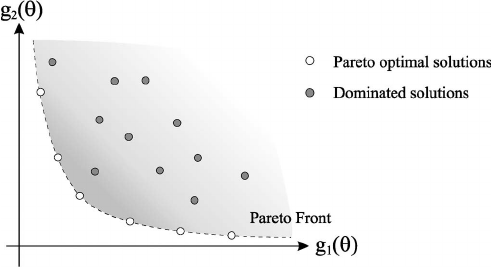
\includegraphics[scale=0.6]{doc/pareto.png}
  \caption{Exemple de solutions paréto-optimales dans un espace à deux objectifs \arthur{Quelqu'un n'aurai pas une meilleure image SVP ?}}
  \label{fig:pareto}
\end{figure}

\subsubsection{Somme pondéré}
Pour se ramener à un problème plus simple, on peut faire une somme des fonction objectif pour se retrouve avec une seule fonction objectif. Et ainsi on peut résoudre le programme linéaire avec un simplexe de manière classique. Cependant, pour pouvoir trouver toutes les solution non dominées, il faut faire cette somme mais en favorisant tour à tour les d'objectifs. Et si on résout toutes les sommes pondérées objectifs avec toutes les combinaisons de poids possibles, on aura alors trouvé toutes les solution paréto-optimales. Seulement les combinaisons de poids sont très nombreuses.

\subsubsection{Cas bi-objectif}\arthur{à refaire}
Dans le cas d'un problème bi-objectif, l'espace des objectifs est un plan et les solutions non dominées forment une ligne que l'on peut explorer d'un bout à l'autre.

\subsubsection{Cas multi-objectif}\arthur{à refaire}
Mais dans le cas multi-objectif, on à trois ou plus objectifs. Donc les solutions non-dominées sont sur un polytope de dimension supérieure à trois. N'ayant plus la possibilité de les explorer d'un bout à l'autre, on les énumères toutes en faisant attention de ne pas recalculer deux fois la même solution.

\subsection{Algorithme de Benson}\arthur{à enlever ?}

\section{Algorithme du simplexe multi-objectif}\arthur{trop conci}

\subsection{idée générale}

Le simplexe multicritère est un algorithme qui énumère toutes les bases non-dominées d'un MOLP (Multi Objective Linear Problem).
Comme on est dans le cas d'un problème linéaire, on sais que toutes les bases non-dominées sont au bord d'un polytope et qu'on peut passer d'une base à une autre par un pivot dit ``efficace''.\\
Un pivot est efficace si le problème auxiliaire construit à partir des fonction objectifs de la base que l'on cherche à atteindre est non borné. L'algorithme consiste donc à explorer tous l'ensemble des solutions à partir d'une seule base (\textbf{phase 3}).\\
La première base non-dominée est calculée par la \textbf{phase 2} Pour cela, on fait une résolution de la somme pondérée du problème. Les poids de cette somme sont calculés lors de la résolution de la variante duale de l'algorithme de Benson.\\
Avant de commencer toute résolution, il faut vérifier que le problème n'est pas impossible, pour cela, on fait une \textbf{phase 1} de simplexe classique.

\textbf{Construction du problème auxiliaire :}\\
Pour savoir si il serait intéressant selon les objectifs de faire entrer une variable $Xj$ dans la base, on construit un problème auxiliaire avec les fonction objectifs de la base courante. On met les colonnes des variables hors base dans une matrice R. On utilise cette matrice dans le PL : la matrice des contraintes est la concaténation de cette matrice R et de moins la colonne j de R,(la colonne de la variable que l'on pense faire entrer dans la base). On construit la fonction objectif de ce problème avec la somme de ses contraintes. Si la résolution de ce problème est bornée, alors introduire la variables j dans la base mènera vers une base non-dominée.

\subsection{Algorithme du simplexe multi-objectif}
\begin{algorithm}[!h]
  \begin{small}
    \BlankLine\DontPrintSemicolon
    \textbf{Phase 1 : phase 1 simplexe classique }\\%\tcc*{On cherche si le problème est dégénéré}}
    La phase 1 du simplexe nous donne une solution admissible $X_0$\\
    \eIf{il n'y a pas de solution admissible}{
      le problème est impossible\\
    }{
      \textbf{Phase 2 : Dual de Benson et première base}\\
      On construit un problème dual de Benson du MOLP \\%avec des variables $u$ devant les anciens coefficients du vecteur $b$ et des variables $w$ devant le vecteur résultant du produit des fonctions objectifs et de la solution $X_0$ trouvée à la phase 1.(On conttraind $w \geq 1$)\\
      \eIf{le dual est impossible}{
        le MOLP est non-borné.
      }{
        On utilise les poids trouvés par le dual de Benson et on résout la somme pondérée\\
        On obtiens une première base non-dominée et on la met dans la liste L\\
        \textbf{Phase 3 : Énumération des bases non-dominées}\\
        On se place sur la première base trouvée à la phase 2\\
        \While{il reste des bases à explorer dans la liste}{
          On utilise la forme révisée du simplexe pour calculer les fonctions objectifs dans la base courante\\
          \For{Chaque variable $X_j$ qui n'est pas en base}{
            On résout problème auxiliaire avec le simplexe\\
            \If{le problème auxiliaire est non borné}{
              La variable est efficace,\\
              On calcul alors la variable sortante grâce à la forme révisée et la décomposition LU\\
              \If{une variable peut sortir}{
                On construit une nouvelle base en interchangeant la variable entrante et la variable sortante\\
                \If{La nouvelle base n'est pas déjà dans la liste L}{
                  On l'ajoute au bout de la liste\\
                }
              }
            }
            On se place sur la base suivante de la liste
          }
          \Retour{Liste L}
        }
      }
    }
  \end{small}
  \caption{\textbf{Multicriteria simplexe Algorithm From Matthias Ehrgott\cite{ehrgott2005multicriteria}}}
\end{algorithm}


\vfill
\break

\vfill
\break

\vfill
\break

\section{Implémentation de l'algorithme}
L'implémentation de l'algorithme précédemment décrit a été réalisé en Julia, version 1.02. Nous allons ici décrire les choix d'implémentations qui on été faits leurs justifications et leurs conséquences.

\subsection{Structure de donnée}\arthur{pas clair ?}
Pour coder les données du problème, on utilise simplement les matrices et les vecteurs de Julia. Ces objets sont indicés à partir de 1 en Julia.\\
\indent Pour résoudre la phase un du simplexe, le dual de benson et la première somme pondérée, on utilise la modélisation JuMP et un solveur, par exemple GLPK.\\
\indent Si les choix d'implémentations ci-dessus paraissent évident, il n'est pas de même pour le choix concernant l'encodage des Bases et des listes de Bases. En effet, L'algorithme tel que décrit dans \cite{ehrgott2005multicriteria} propose deux listes L1 et L2. Les bases que l'on a trouvées mais pas encore explorées sont dans la liste L2 et quand on a détecté toutes les variables efficaces de cette base, on   la retire de L2 pour la mettre dans L1. Lors de l'algorithme, quand on trouve une nouvelle base, avant de l'ajouter à la liste L2, on doit vérifier qu'elle n'appartient pas déjà à aucune des listes en prenant en compte que la base peut être dans un autre ordre. On a donc ici une représentation ensembliste des bases. Il existe en julia une telle classe d'objet, les set qui on été testés dans les premières implémentations. On avais alors des bases qui étaient des ensembles de variables et des liste qui étaient des ensembles de bases.\\
\indent Cependant, l'implémentation s'est dirigée vers une structure plus simple les tableaux. Cette implémentation a deux avantages par rapport aux set, on connais sa complexité et elle permet de ne manipuler qu'une seule liste. En effet comme un tableau est indicé, cela nous permet de passer simplement sur la base suivante du tableau et d'ajouter les nouvelles bases au bout de celui-ci. Pour savoir si une base appartient à la liste, on est obligé de regarder une à une les variables de chaque bases de la liste. On a donc une complexité de $\mathcal{O}(\#(B)^2 \times \#(L))$.\\
Une deuxième idée pour gagner en complexité serai de trier les bases. De cette manière, on peut savoir plus simplement si elles appartiennent à la liste de bases. Cette structure a théoriquement une complexité de $\mathcal{O}(\#(B\times log(B))+\#(B)\times \#(L))$ Même si dans la pratiques les deux approches sont équivalentes en terme de temps d'exécution car la principale complexité de l'algorithme est dans la résolution des problèmes auxiliaires et des systèmes d'équations de la décomposition LU.

\subsection{Comparaison des implémentations et observations}
Lors de l'implémentation, une erreur dans la décomposition LU a forcé la réécriture de la phase trois avec la matrice inverse de la forme révisé du simplexe pour vérifier les calculs. Comme dit précédemment, la décomposition LU permet de simplifier les calculs et d'accumuler moins d'imprécisions numériques. Cette observation est flagrante lors des tests même si sur les grandes instances, la décomposition LU peut générer quelques erreurs d'imprécisions numériques.
Pour les tests, une matrice arrondissant la matrice du problème auxiliaire à été écrite. Elle est lourde en complexité temporelle mais elle permet d'éviter quelques erreurs.\\

%On observe que surprenemment, même si on fais des arrondis sur les matrices R et qu'on ne tri pas les bases, on obtiens deux matrices R différentes dans la base [5, 3] de l'exemple ZELENY 3-8. Alors que seule la méthode change. Cette différence est unique et très surprenante.\\
\subsection{Instances}
\subsubsection{Générateur d'instances}
La génération de problèmes aléatoires est dirigée par plusieurs paramètres qui peuvent êtres modifiés.

Notation :
\begin{itemize}
\item $[a:b]$ signifie toutes les valeurs entières entre $a$ et $b$ inclus.
\end{itemize}

Pour les paramètres :
\begin{itemize}
\item $[3:9]$ objectifs,
\item $[2:20]$ variables,
\item $[1:30]$ contraintes,
\item $[-9:9]$ pour les valeurs dans A et C avec une forte probabilité pour la valeur 0
\item $[1:20]$ pour les valeurs de b
\item une chance sur 6 d'avoir une contrainte d'égalité et le reste des chances réparties entre les inégalités
\end{itemize}

\subsubsection{Observations}
On remarque que 70\% des instances générés sont impossibles, 25\% des restantes ne passent pas la phase 2 et quand le problème n'est pas dégénéré, il est rare de ne pas avoir plusieurs rayons infini lors de l'exploration des bases. On en déduit qu'il est très difficile de générer des instances possibles et intéressantes. Quelques exemples générés intéressants sont dans le fichier resultats.jl

\subsubsection{Parser d'instances}
Pour tester d'autres instances, un parser pour les instances .mop a été fais. \\
Exemple d'instance qui peut être parsé : "data/molp\_10\_779\_10174\_entropy.mop"

\section{Pistes d'améliorations}
\subsection{Récupération de la première base dans JuMP ou GLPK}
Pour l'instant, l'algorithme fais une hypothèse de non-dégénérescence pour déterminer la première base à la fin de la phase 2. Cette hypothèse est très dérangeante car la majorité des instances existantes sont dégénérées.
\subsection{Interface avec voptgeneric}
L'interface avec vopt reste à faire mais la mise a jour en cour de JuMP vers sa version 19 rend ceci compliqué.
\subsection{Optimisation}
On pourrait peut-être gagner un peu temps en reprogrammant la résolution des systèmes triangulaires (sup et inf) si elle n'est pas traitée spécifiquement dans Julia. Mais sinon, l'implémentation tableau semble être la plus optimisée pour la phase 3, à voir si on peut faire des choses combinées avec vOpt pour la phase une et deux. \\
Peut-être que d'autres structures qu'un tableau pourraient être utilisées mais elles ne paraissent pas très convaincantes lors des premières implémentations.
\subsection{Interprétation graphique}
L'algo nous donne les bases et les solution donc on peu recalculer les coûts mais il faudrait un petit traitement pour reconnaître les bases qui forment des faces non dominées pour apporter une réponse graphique.



\section{Instances}
Les instances utilisés dans ce projet sont tirées des livres suivants :\cite{ehrgott2005multicriteria}, \cite{steuer1986multiple}, \cite{zeleny1973multiple}

\begin{figure}[htb!]
  \centering
  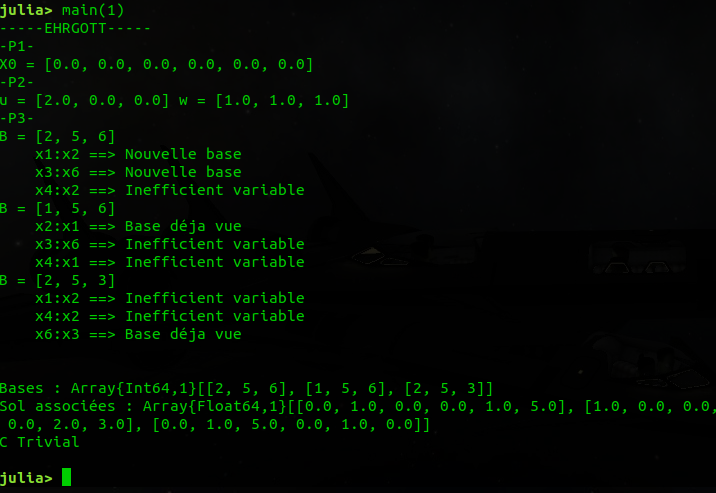
\includegraphics[scale=0.5]{doc/Ehrgott.png}
  \caption{Exemple d'exécution sur l'instance du livre de Matthias Ehrgott\cite{ehrgott2005multicriteria}}
  \label{fig:Ehrgott}
\end{figure}


\vfill
\break

\section{Multicriteria simplexe Algorithm : Pseudocode formel}
Cette section propose une écriture plus formelle de l'algorithme. Comme Julia est un langage de programmation de haut niveau, l'implémentation est très proche de cette écriture.
\subsection*{Nomenclature}
\begin{itemize}
\item MOLP : $ min \{ Cx : Ax + Iz = b,x,z \geq 0 \} $
\item $C$ : matrice des fonctions objectifs
\item $A$ : matrice des contraintes
\item $b$ : vecteur des membres de droite des contraintes
\item $x$ : variables
\item $z$ : variables d'écarts\\
  \textbf{Phase 1}
\item $e$ : vecteur null
\item $x^0$ : solution de la phase 1\\
  \textbf{Phase 2}
\item Dual du MOLP : $min \{ u'b + \lambda'Cx^0 : u'A + \lambda'C \geq 0,\lambda \geq e \} $
\item $u$ : variables duales associées au vecteur b
\item $\lambda$ : variables duales associées au fonction objectifs
\item $e$ : vecteur de 1
\item $\lambda_1$ : poids trouvés après la résolution du dual. Ils sonts utilisés dans la première somme pondérée
\item $B1$ : première base
\item $x1$ : première solution
\item $LB$ : liste des bases
\item $Lx$ : liste des solutions\\
  \textbf{Phase 3}
\item cb : indice de la base courante
\item $B$ base courante
\item $\omega$ : ensemble des variables
\item $N$ : variables hors bases
\item $A_B$ : Matrice A avec seulement les colonnes des variables en bases
\item L,U : décomposition en une matrice triangulaire inférieure et une matrice triangulaire supérieure de la matrice $A_B$
\item $k$ : indice de la fonction objectif
\item $C_B[k]$ : Coefficients de la fonction objectif $k$ dans la base $B$
\item $A_N$ : Matrice A avec seulement les colonnes des variables hors bases
\item $C_N[k]$ : Coefficients de la fonction objectif $k$ des variables hors bases
\item $R$ : matrice des coefficients des fonctions objectifs obtenus par la forme révisée et la décomposition LU
\item PL auxiliaire : $min \{ e'(y+\delta) : Ry - r^j\delta + Iv = 0,y,\delta,v \leq 0 \}$ PL qui donne l'efficacité d'une variable
\item $r^j$ : colonne j de la matrice $R$
\item $e$ : vecteur de la somme des colonnes de la matrice $concat(R,-r^j)$
\item $x_b$ : solution associée à la base $B$
\item $x^s$ : variable sortante
\item $Bj$ : nouvelle base
\item $x_j$ : nouvelle solution associée à la base $Bj$
\end{itemize}

\subsection*{Algorithme}
\begin{algorithm}[!h]
  \begin{small}
    \SetKwIF{Si}{SinonSi}{Sinon}{Si}{alors}{Sinon si}{alors}{fin si}{}
    \BlankLine\DontPrintSemicolon
    \textbf{Phase 1 : phase 1 simplexe classique \tcc*{mono-objective simplexe Phase 1}}
    Solve $ min \{ e'z : Ax + Iz = b,x,z \geq 0 \} $\\
    \eIf{z == 0}{
      $x^0$ is a basic solution of the MOLP\\
    }{
      $ X = \oslash $\tcc*{the MOLP is infeasible}
    }
    \textbf{Phase 2 : Benson Dual and first basis}\\
    Solve $ min \{ u'b + \lambda'Cx^0 : u'A + \lambda'C \geq 0,\lambda \geq e \} $\tcc*{dual simplexe gives us the first wheights:$\lambda_1$}
    \eIf{:Infeasable}{
      $ X_E = \oslash $\tcc*{The MOLP has no efficients solutions}
    }{
      Solve $ min \{ \lambda_1'Cx : Ax = b,x \geq 0 \} $\tcc*{the first weighted sum gives us the first non-dominated Basis}
      Find basis $B1$ and solution $x1$\\
      $LB := B1$ and $Lx := x1$ \tcc*{we put them in a list of basis to explore, and a list of solution}
    }
    \textbf{Phase 3 : Basis enumaration}\\
    cb = 1 \tcc*{index of the curent basis}
    \While{$cb \leq length(LB)$}{
      $B = LB[cb]$ and $x_b = Lx[cb]$\tcc*{while we have basis to explore in the list}
      $N = \Omega - B$\tcc*{N:non-basis variables ($\Omega$:all variables)}
      L,U = LU décomposition of $A_B$\tcc*{LU decomposition of matrix A on basis B}
      \For{$k \leftarrow 1$ \KwTo number of objectives }{
        Solve $t'U = C_B[k]$\tcc*{calcul des objectifs par la forme révisée du simplexe et la décomp LU}
        Solve $y'L = t'$\\
        $R[k] = (C_N[k])' - y'A_N$\tcc*{R is the matrix of the non-basic vars of the objectives fonctions}
      }
      \For{$j \leftarrow 0$ \KwTo length(N)}{\tcc*{for all variable in N, we test if there are efficient with the following PL}
        Solve $min \{ e'(y+\delta) : Ry - r^j\delta + Iv = 0,y,\delta,v \leq 0 \}$\\
        \eIf{:Unbounded}{
          ``Inefficient variable''
        }{
          Solve $Ly = x_b$\tcc*{revised simplexe + LU decomp}
          Solve $Ud = y$\\
          s = find positive min $\frac{x_b}{d}$\tcc*{$x^s$:variable out of the pivot}
          \eIf{s doesn't exist}{
            ``Impossible Pivot or infinite ray''
          }{
            ``Pivot Xj:Xs''\\
            $Bj$ new basis and $x_j$ new solution\\
            \eIf{$Bj$ is already in $L$}{
              ``already known Basis''\tcc*{with 3 or more objectives, we can return on old basis}
            }{
              $LB := Bj$ and $Lx := x_j$\tcc*{we add the new basis and the new solution to the lists}
            }
          }
        }
      }
      cb = cb + 1      
    }
    \Retour{Liste L}
  \end{small}
  \caption{\textbf{Multicriteria simplexe Algorithm From Matthias Ehrgott\cite{ehrgott2005multicriteria}}}
\end{algorithm}

\break
\vfill

\break
\vfill

\break
\vfill

\break
\vfill

\section{Conclusion}
Nous avons tout d'abord cherché à implémenter l'algorithme tel que décrit dans \cite{ehrgott2005multicriteria}. Nous avons remarqué que celui-ci pouvait être légèrement optimisé en modifiant les structures de données qu'il utilise.\\
\indent Puis nous avons amélioré l'algorithme avec la forme révisée du simplexe et la décomposition LU. Et nous avons obtenu une réduction conséquente des imprécisions numériques.\\
\indent Nous avons observé qu'un générateur d'instance peine à créer des problèmes intéressants. Il nous est aussi difficile de parser des instance à cause de l'hypothèse de non-dégénérescence de la phase 2. L'idéal aurai été de la récupérer directement de la modélisation de JuMP mais cette opération restera très incertaine tant que sa version ne sera pas stable.\\
\indent C'est pour cette même raison que l'intégration de l'algorithme à vOptSolver n'a pas été faite.\\
\indent L'interface graphique pourrait être intéressante mais elle ne parais pas vitale pour cet algorithme car il ne sera pas utilisé en tant que tel. En effet, il existe peu de problèmes molti-objectif linéaires et continus. L'utilisation de cet algorithme parais plus utile dans la relaxation d'un problème multi-objectif combinatoire. De ce fait, l'algorithme se doit d'être le plus optimisé possible. Et pour ceci, les deux pistes que nous avons sont la reprogrammations de la décomposition LU d'une matrice et de la résolution des systèmes d'équations triangulaires. Car on ne sais pas si ces méthodes implémentées en Julia correspondent exactement à notre problème.

%\break
%\vfill

\bibliographystyle{plain}
\bibliography{biblio}

\end{document}

